\documentclass[twocolumn]{article}
\usepackage[spanish]{babel}
\usepackage[utf8]{inputenc}
\usepackage{amssymb}
\usepackage{graphicx}
\usepackage{verbatim}
\usepackage{algorithmic}
\usepackage{tabu}
\usepackage{color}
\usepackage{xcolor}
\usepackage{listings}
\usepackage{enumitem}
\usepackage{multicol}
\usepackage{tikz-qtree}
\usepackage{enumitem}
\setlist{nolistsep}


\author{
Nombre:....................................... \\
    Departamento de Informática y Sistemas \\
    Universidad EAFIT \\
}
\title{
    Estructuras de Datos 1 - ST0245 \\
    Examen Parcial 2 - 032 - Martes
}
\date{
    Octubre 24 de 2017
}

\begin{document}
\vspace{-5cm}
\maketitle


\section*{Criterios de calificación}


\begin{itemize}
\item Selección múltiple con única respuesta
\begin{itemize}
\item Respuesta correcta: 100\%
\item Respuesta incorrecta: 0\%
\end{itemize}

\item Completar código
\begin{itemize}
\item Respuesta correcta 100\%
\item Respuesta incorrecta o vacía 0\%\\
\end{itemize}
\end{itemize}


\textbf{NOTAS IMPORTANTES:}
\begin{itemize}
	\item Responda en la hoja de PREGUNTAS
	\item Marque la hoja de PREGUNTAS
\end{itemize}


\section{Árboles binarios 30\%}
Dado un árbol $n -ario$, un camino desde la raíz a cualquiera de sus hojas se considera \textbf{simple} si la suma de sus elementos pares es igual a la suma de sus elementos impares. Por ejemplo, un camino desde la raiz hasta una hoja con los elementos [1, 2, 1] es \textbf{simple}, pero el camino desde la raíz hasta una hoja [1, 3, 1] \textbf{no es simple}. Su tarea es determinar cuantos caminos \textbf{simples} hay en un árbol. La implementación de un nodo $n-ario$ es la siguiente:

\begin{verbatim}
class NNodo{
  int val; //Valor en el nodo actual.
  //Hijos del nodo actual.
  LinkedList<NNodo> hijos; 
}
\end{verbatim}

\begin{center}
  \begin{tikzpicture}
\Tree
[.1
  [.4
    [.7
    ]
    [.9
    ]
    [.3
    ]
  ]
  [.13
    [.11
    ]
    [.14
    ]
  ]
  [.11
    [.4
    ]
    [.3
    ]
  ]
  [.8
    [.6
    ]
    [.7
    ]
  ]
  [.1
    [.2
    ]
  ]    
]
\end{tikzpicture}
\end{center}

(10\%) ¿Cuantos caminos \textbf{simples} hay desde una raíz hasta una hoja en el árbol anterior?
\begin{enumerate}[label=\Alph*]
\item 1
\item 2
\item 3
\item 4 \\
\end{enumerate}


El siguiente código nos ayuda a determinar el numero de caminos simples en un árbol, pero faltan algunas lineas. Completa las lineas que faltan.

{\small
\begin{verbatim}
01 public int cuantosSimples(NNodo raiz, int suma){
02  //Arbol vacio 
03  if(raiz ==  null)
04    ______________;
05  //Hoja
06  if(raiz.hijos.size() _______) // Si suma es 0
07    return  (suma == 0) ? 1 : 0; // Retorne 1, sino, 0
08  int total = 0;
09  for(NNodo n: raiz.hijos)
10    if(n.val % 2 == 0) // Par
11      total += cuantosSimples(n, suma + n.val);   
12    else // Impar
13      total += cuantosSimples(n, suma - n.val);   
15  return total;
16 }
17
18 public int cuantosSimples(NNodo raiz){
19  int val = (raiz.val % 2 == 0) ? 
              raiz.val : -raiz.val;
20  return cuantosSimples(raiz, val);
21 }
\end{verbatim}
}

 (10\%) Complete la linea 4 \hrulefill

 (10\%) Complete la linea 6 \hrulefill



%\clearpage
\section{Implementación grafos 10\%}
Considere el siguiente grafo:

\begin{center}
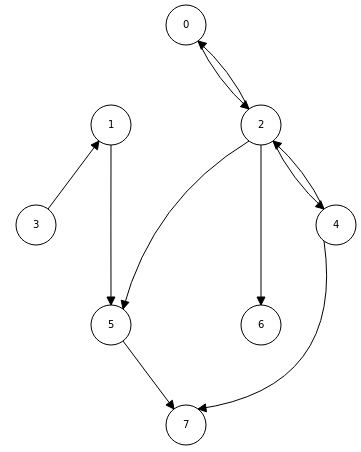
\includegraphics[scale=0.5]{grafin.png}
\end{center}

 Complete la representación de \textbf{matrices de adyacencia}. Si no hay arco,
  por simplicidad, deje el espacio en blanco. No coloque ceros.

\begin{center}
\begin{tabular}{| c | c | c | c | c | c | c | c | c |}
\hline
  & 0 & 1 & 2 & 3 & 4 & 5 & 6 & 7 \\
\hline
0 &   &   & 1  &  &   &   &   &   \\
\hline
1 &   &   &   &   &   & 1  &   &   \\
\hline
2 &   &   &   &   &   &   &   &   \\
\hline
3 &   &   &   &   &   &   &   &   \\
\hline
4 &   &   &   &   &   &   &   &   \\
\hline
5 &   &   &   &   &   &   &   &   \\
\hline
6 &   &   &   &   &   &   &   &   \\
\hline
7 &   &   &   &   &   &   &   &   \\ 
\hline
\end{tabular}
\end{center}

\section{Colas 20\%}

En el juego de \textit{hot potato} (conocido en Colombia como \textit{Tingo, Tingo, Tango}), los niños
hacen un círculo y pasan al vecino de la derecha, un elemento,
 tan rápido como puedan. En un cierto punto del juego,
 se detiene el paso del elemento. El niño que queda con el
 elemento, sale del círculo. El juego continúa
 hasta que sólo quede un niño.

 Este problema se puede simular usando una cola. El algoritmo
 tiene dos entradas: Una cola \texttt{q}  con los nombres de los niños y una constante entera \texttt{num}. El algoritmo retorna el nombre de la última persona que queda en el juego, después de pasar la pelota, en cada ronda, \texttt{num} veces. Como un ejemplo, para el círculo de niños \textit{[Brad, Kent, Jane, Susan, David, Bill]},
donde \textit{Bill} es el primer niño y \textit{Brad} es el último,
y \texttt{num} es igual a 7, la respuesta es \textit{Susan}. Cada niño pasa la pelota al niño que tiene a su derecha.


 En Java, el método \texttt{add} agrega un elemento
 al comienzo de una cola, y el método \texttt{remove} retira un elemento del final de una cola y retorna el elemento.


{\small
\begin{verbatim}
01 String hotPotato(Queue<String> q, int num) {
02   while (q.size() > 1) {
03      for (int i = 1; i <= num; i++) 
04         q.add(q.remove()); 
05      q.remove(); }
06   return q.remove(); }
\end{verbatim}
}

¿Cuál es la complejidad asintótica del método \texttt{hotPotatoe},en el peor de lso casos, asumiendo que el número inicial de niños en la cola es $n$ y el número de de veces que se pasa la pelota
en cada ronda es $num$? \\

O(\_\_\_\_\_\_\_\_\_\_\_\ )

%O(n*num)

\section{Árbol de busqueda 20\%}
 Se van a ingresar los elementos $[3, 7, 8, 6, 4, 1, 9, 2]$ en un arbol binario de busqueda en su orden, es decir, primero el 3, segundo el 7, tercero el 8 y así sucesivamente. 

 (10\%) ¿Cuáles son los numeros que van en las posiciones $a, b, c, d, e$ respectivamente en el siguiente árbol.
\\
\begin{center}
\begin{tikzpicture}
\Tree
[.3     
    [.a
      \edge[]; \node[]{};
      [.2
      ]
    ]
    [.b  
      [.6
        [.e
        ]
        \edge[]; \node[]{};
      ]
      [.c
        \edge[]; \node[]{};
        [.d
        ]     
      ]
    ]
]
\end{tikzpicture}
\end{center}

\begin{enumerate}[label=\Alph*]
\item 1, 7, 8, 9, 4
\item 1, 4, 7, 8, 9
\item 4, 1, 7, 9, 8
\item 1, 9, 8, 4, 7 \\
\end{enumerate}

(10\%) Un recorrido in-orden está representado por el siguiente
algoritmo:

\begin{verbatim}
void InOrden(Node node){
 if (node != null){
   InOrden(node.left);
   System.out.println(node.data);
   InOrden(node.right);
} }
\end{verbatim}

¿Cuál es el recorrido in-orden del árbol anterior?
\begin{enumerate}[label=\Alph*]
\item 1, 3, 2, 4, 6, 7, 9, 8
\item 1, 2, 3, 4, 6, 7, 8, 9
\item 2, 1, 4, 6, 9, 8, 7, 3
\item 3, 1, 2, 7, 6, 4, 8, 9
\end{enumerate}



\section{Pilas 30\%}

En la vida real, una tarea de los compiladores es determinar si los paréntesis de un
código fuente están correctamente balanceados. En el curso \emph{Lenguajes Formales y Compiladores} podrán
profundizar sobre ese tema. Para efectos de este curso, ese problema puede resolverse usando pilas.

A Benito le piden escribir un programa, usando pilas, que recibe una cadena que contiene paréntesis. El programa debe determinar, usando una pila, si están correctamente balanceados;
es decir, si se abren y cierran correctamente. El programa ignora los caracteres que no sean paréntesis. Como un ejemplo, para esta entrada $((2+2)*(3+3))-(3-4)$ debe retornar verdadero y 
para esta entrada $(5-((3+3)$ debe retornar falso. Ayúdele a Benito a completar su programa.

{\small
\begin{verbatim}





01 public class Parentheses {
02  private static final char L_PAREN = '(';
03  private static final char R_PAREN = ')';
04  public static boolean isBalanced(String s) {
05   Stack<Character> stack = new Stack<Character>();
06   for (int i = 0; i < s.length(); i++) {
07     if (s.charAt(i) == L_PAREN)   
08         stack.push(_____);
09     else if (s.charAt(i) == R_PAREN) {
10         if (stack.isEmpty())        return ___;
11         if (stack.pop() != L_PAREN) return ___;
12     }
13   }
14    return stack.isEmpty();
15  }
16 }
\end{verbatim}
}

En Java, la palabra \texttt{final} se usa para definir una constante, es decir, 
una variable cuyo valor no se puede cambiar. Para pilas en Java,
el método \texttt{push()} ingresa un elemento a la pila, el método \texttt{pop()}
saca un elemento de pila, y el método \texttt{isEmpty()} retorna verdadero si 
una pila está vacía y falso de lo contrario. Finalmente, para cadenas
de caracteres en Java, el método \texttt{charAt(i)} retorna el caracter que se
encuentra en la posición \texttt{i} de una cadena de caracteres. \\

(10 \%) Complete el espacio en la línea 08.\\

\_\_\_\_\_\_\_\_\_\_\_\ 

(10 \%) Complete el espacio en la línea 10.\\

\_\_\_\_\_\_\_\_\_\_\_\ 

(10 \%) Complete el espacio en la línea 11.\\

\_\_\_\_\_\_\_\_\_\_\_\ 

% 01 public class Parentheses {
% 02  private static final char L_PAREN    = '(';
% 03  private static final char R_PAREN    = ')';
% 04  public static boolean isBalanced(String s) {
% 05    Stack<Character> stack = new Stack<Character>();
% 06    for (int i = 0; i < s.length(); i++) {
% 07        if      (s.charAt(i) == L_PAREN)   
% 08            stack.push(L_PAREN);
% 09        else if (s.charAt(i) == R_PAREN) {
% 10            if (stack.isEmpty())        return false;
% 11            if (stack.pop() != L_PAREN) return false;
% 12        }
% 13    }
% 14    return stack.isEmpty();
% 15  }
% 16 }

\end{document}
